
\section*{Introduction à deux problèmes en communication numérique}
\section{Introduction}
On s'intéresse au problème de communication entre deux personnes, nommées Alice et Bob qui cherchent à s'envoyer un message au travers d'un canal de communication (une bande de fréquences radio par exemple).

Avant d'être lu par Bob, le message original d'Alice passe par plusieurs étapes que nous allons séparer de la manière suivante :

\begin{itemize}
  \item une phase de compression, durant laquelle Alice cherche à trouver la représentation la plus compacte possible du message,
  \item une phase d'encodage durant laquelle le message compressé est transformé en une succession de symboles transmissibles au travers du canal de communication utilisé,
  \item une phase de transmission durant laquelle le message encodé circule sur le canal de communication et est susceptible de subir une altération,
  \item une phase de décodage durant laquelle Bob décode le message qu'il a reçu, le message lui apparaît alors sous la forme compressée,
  \item une phase de décompression durant laquelle Bob applique l'opération réciproque de la compression opérée par Alice.\\
\end{itemize}

Ce modèle est décrit par le schéma de la Figure \ref{fig_ccmp_2024_info_01}.

\begin{figure}[!h]
\centering
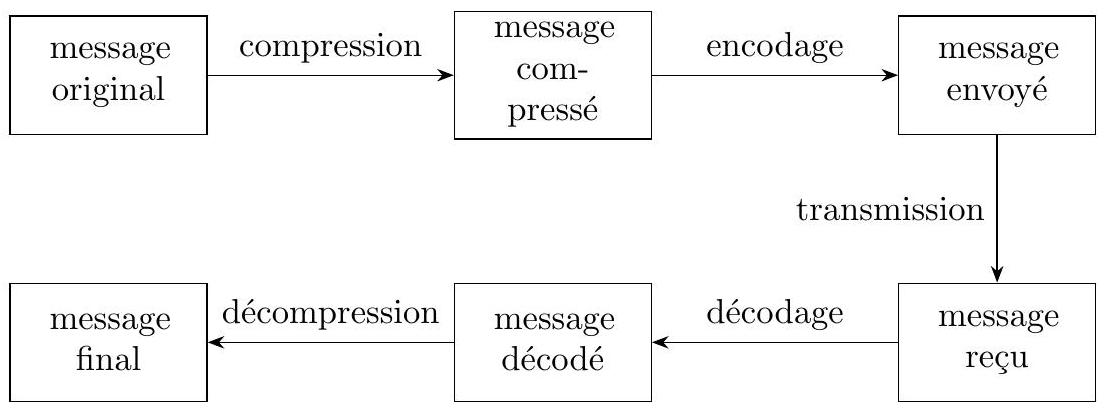
\includegraphics[max width=.8\textwidth]{2025_04_25_b5f58c3e8cc704f29fe4g-02}
\caption{Schématisation du modèle de communication considéré ici.\label{fig_ccmp_2024_info_01}}
\end{figure}

Dans cette épreuve, nous allons nous intéresser uniquement à deux phases : la compression du message d'origine par Alice en un message compact et le décodage par Bob d'un message transmis, potentiellement entaché d'erreurs.

\section{Compression du message d'Alice : codage arithmétique}
Le codage ASCII (American Standard Code for Information Interchange) définit une norme où 128 caractères sont codés sur 7 bits. Ce codage est illustré par les quelques lignes suivantes :

\begin{center}
\begin{tabular}{ccc}
\hline
\textbf{Caractère} & \textbf{Codage binaire} & \textbf{Équivalent numérique} \\
\hline
\lstinline{'a'} & 1100001 & 97 \\
\hline
\lstinline{'b'} & 1100010 & 98 \\
\hline
\lstinline{'z'} & 1111010 & 122 \\
\hline
\end{tabular}
\end{center}

Lorsqu'une chaîne de caractères n'utilise pas l'intégralité des 128 caractères proposés par le codage ASCII, il est possible de convenir d'une représentation différente, plus économique en nombre de symboles. Considérons la chaîne de caractères $s=$ 'abaabaca'. On peut proposer de coder celle-ci à l'aide du tableau suivant :

\begin{center}
\begin{tabular}{cc}
\hline
\textbf{Caractère} & \textbf{Code}\\
\hline
\lstinline{'a'} & 00 \\
\hline
\lstinline{'b'} & 01 \\
\hline
\lstinline{'c'} & 10 \\
\hline
\end{tabular}
\end{center}

Dans ce cas, la chaîne de caractères s est codée sur 16 bits par :

$$
00 \quad 01000001001000
$$

(où des espaces ont été introduits pour faciliter la lecture).\\
Dans un souci de compression de l'information, il est intéressant de représenter les caractères les plus fréquents par des expressions courtes et de ne plus nécessairement coder avec des codes de longueur constante chaque caractère. Dans l'exemple précédent, il est possible de coder le caractère \lstinline{'a'} avec 1 bit, et les caractères \lstinline{'b'} et \lstinline{'c'} avec 2 bits afin de coder la chaîne s sur seulement 11 bits en tout.

\question{Proposer une telle représentation en expliquant pourquoi celle-ci pourra être décodée sans ambiguïté. Vous ferez en sorte que la représentation binaire de \lstinline{'a'} soit inférieure à celle de \lstinline{'b'}, elle-même inférieure à celle de \lstinline{'c'}.}

La représentation précédente emploie la même longueur pour coder les caractères \lstinline{'b'} et \lstinline{'c'} alors que le caractère \lstinline{'b'} est deux fois plus présent que le caractère \lstinline{'c'} dans la chaîne \lstinline{s}.

Il est possible d'aller un cran plus loin et le codage arithmétique présenté dans cette étude permet un gain de compression comme s'il parvenait à représenter un caractère avec un nombre non entier de bits au prorata de sa fréquence d'apparition.\\
Ce principe de compression est notamment utilisé par la norme JPEG2000 de compression des images. Nous ne le présenterons cependant ici que dans le cadre de l'étude de chaînes de caractères.

\subsection{Analyse du texte source}
L'objet de cette partie est d'analyser le contenu d'une chaîne de caractères s afin de déterminer :

\begin{itemize}
  \item les caractères utilisés par la chaîne \lstinline{s};
  \item le nombre d'occurrences de chacun.
\end{itemize}

\question{Écrire une fonction nommée \lstinline{nbCaracteres(c:str,s:str) -> int} qui prend comme argument un caractère \lstinline{c}, une chaîne \lstinline{s} et qui renvoie le nombre d'occurrences (c'est-à-dire le nombre d'apparitions) de \lstinline{c} dans \lstinline{s} . La fonction doit avoir une complexité linéaire en $n$ , la longueur de la chaîne \lstinline{s}.}

\question{Pour déterminer la liste des caractères utilisés à l'intérieur d'une chaîne s on utilise la fonction définie ci-dessous :}

\begin{lstlisting}
def listeCaracteres(s:str):
    listeCar = []
    n = len(s)
    for i in range(n):
        c = s[i]
        if not(c in listeCar):
            listeCar.append(c)
    return listeCar
\end{lstlisting}

Que renvoie cette fonction lorsque \lstinline{s='abaabaca'} ? Expliquer succinctement le principe de fonctionnement de cette fonction.

\question{En fonction de la longueur n de la chaîne et du nombre k de caractères distincts dans celle-ci, déterminer la complexité asymptotique dans le pire des cas de la fonction de la question Q3. Par exemple pour \lstinline{'abaabaca'}, on a $n=8$ et $k=3$. On négligera la complexité des append mais pas celle des tests d'appartenance de la forme \lstinline{i in L}. Autrement dit, la ligne 7 est considérée comme étant de complexité constante et la ligne 6 de complexité linéaire en la longueur de la liste \lstinline{listeCar}.}

\question{On définit alors une fonction \lstinline{analyseTexte(s:str) -> list}.}
\vspace{-.25cm}
\begin{lstlisting}
def analyseTexte(s:str):
    R = []
    l = listeCaracteres(s)
    for i in range(len(l)):
        c = l[i]
        R.append((c,nbCaracteres(c,s)))
    return R
\end{lstlisting}

\textit{Expliquer ce que fait cette fonction et donner la valeur renvoyée par la commande \lstinline{analyseTexte('babaaaabca')}.}

\question{En fonction de la longueur $n$ de \lstinline{s} et du nombre \lstinline{k} de caractères distincts présents dans \lstinline{s}, (autrement dit \lstinline{k} est la longueur de \lstinline{listeCaracteres(s)}), donner une estimation de la complexité asymptotique dans le pire des cas de la fonction \lstinline{analyseTexte}.}

\question{Adapter la fonction de la question Q5 pour qu'elle utilise (et renvoie) un dictionnaire. Elle devra avoir une complexité} 
\textit{\begin{itemize}
\item linéaire en la longueur $n$ de \lstinline{s};
\item indépendante de $k$ nombre de caractères distincts présents dans \lstinline{s}.
\end{itemize}}

De plus, cette fonction devra impérativement ne parcourir qu'une seule fois la chaîne de caractères. On admettra qu'un test d'appartenance d'une clé à un dictionnaire se fait à coût constant. Par exemple, \lstinline{analyseTexte('abracadabra')} renverra \{\lstinline{'a':5, 'b':2, 'r':2, 'c':1, 'd':1}\}.

\subsection{Exploitation d'analyses existantes}
On peut éviter de réaliser une analyse de la chaîne de caractères à coder en exploitant des données statistiques disponibles. La numérisation de larges corpus littéraires a permis la création de bases de données contenant des informations relatives au nombre d'occurrences des différents caractères alphanumériques dans diverses langues. Nous allons supposer disposer d'une base de données constituée de trois tables (les clefs primaires sont soulignées) :

\begin{itemize}
  \item \lstinline{caractere(idCar, symbole, typeCaractere, codeHTML)};
  \item \lstinline{corpus(idLivre, titre, auteur, annee, nombreCaracteres, langue)};
  \item \lstinline{occurrences(idCar, idLivre, nombreOccurrences)};\\
dont voici quelques extraits :\\
Table caractere :
\end{itemize}

\begin{center}
\begin{tabular}{|c|c|c|c|}
\hline
idCar & symbole & typeCaractere & codeHTML \\
\hline\hline
65 & 'A' & 'lettre' & '\&\#65;' \\
48 & '0' & 'nombre' & '\&\#48;' \\
\end{tabular}
\end{center}

Table corpus :

\begin{center}
\begin{tabular}{|c|c|c|c|c|c|}
\hline
idLivre & titre & auteur & annee & nombreCaracteres & langue \\
\hline\hline
1 & 'Germinal' & 'Zola' & 1885 & 1152365 & 'Français' \\
2 & 'Les Misérables' & 'Hugo' & 1862 & 2245300 & 'Français' \\
\end{tabular}
\end{center}

Table occurrences :

\begin{center}
\begin{tabular}{|c|c|c|}
\hline
idCar & idLivre & nombreOccurrences \\
\hline\hline
62 & 31 & 155 \\
37 & 21 & 1550 \\
\end{tabular}
\end{center}

\question{Écrire en langage SQL une requête permettant d'obtenir la liste sans doublon des auteurs présents dans la table corpus.}

\question{Écrire une requête SQL permettant d'obtenir la fréquence d'occurrences (donc comprise entre 0 et 1) de chaque caractère en 'Français'. Plus précisément, la requête 
devra renvoyer une table à deux attributs : une colonne contenant le symbole de chaque caractère, et une autre colonne contenant le rapport entre le nombre total d'occurrences du caractère et le nombre total de caractères des textes de tout le corpus.}

\subsection{Compression}
La compression par codage arithmétique consiste à représenter une chaîne de caractères s par un nombre réel déterminé à l'intérieur de l'intervalle $[0 ; 1[$.

Initialement, on attribue à chaque caractère utile une portion de l'intervalle $[0 ; 1[$ proportionnelle à sa fréquence d'occurrences. Par exemple, pour un alphabet à 5 lettres 'abcde', on pourrait avoir un tableau comme ci-dessous :

\begin{center}
\begin{tabular}{lccccc}
\hline
\textbf{Caractère} & \lstinline{'a'} & \lstinline{'b'} & \lstinline{'c'} & \lstinline{'d'} & \lstinline{'e'} \\
\hline
\textbf{Fréquence} & 0.2 & 0.1 & 0.2 & 0.4 & 0.1 \\
\hline
\textbf{Intervalle} & $[0 ; 0.2[$ & $[0.2 ; 0.3[$ & $[0.3 ; 0.5[$ & $[0.5 ; 0.9[$ & $[0.9 ; 1[$ \\
\hline
\end{tabular}
\end{center}

La chaîne de caractères \lstinline{s} est codée en partant de l'intervalle $[0 ; 1[$. À chaque caractère successif de celle-ci, on affine cet intervalle en ne considérant que la portion correspondant au caractère lu.

Si par exemple la chaîne à coder est \lstinline{s= 'dac'} :

\begin{itemize}
  \item on obtient d'abord l'intervalle $[0.5; 0.9 [$ correspondant au caractère \lstinline{'d'};
  \item le caractère \lstinline{'a'} détermine alors le sous-intervalle $[0.50 ; 0.58[$ de $[0.5 ; 0.9[$ correspondant à la portion associée au caractère \lstinline{'a'}.
  \item le caractère \lstinline{'c'} détermine enfin l'intervalle $[0.524; 0.540[$.
\end{itemize}

La figure \ref{fig_ccmp_2024_info_02} qui suit illustre ce processus.

\begin{figure}
\centering
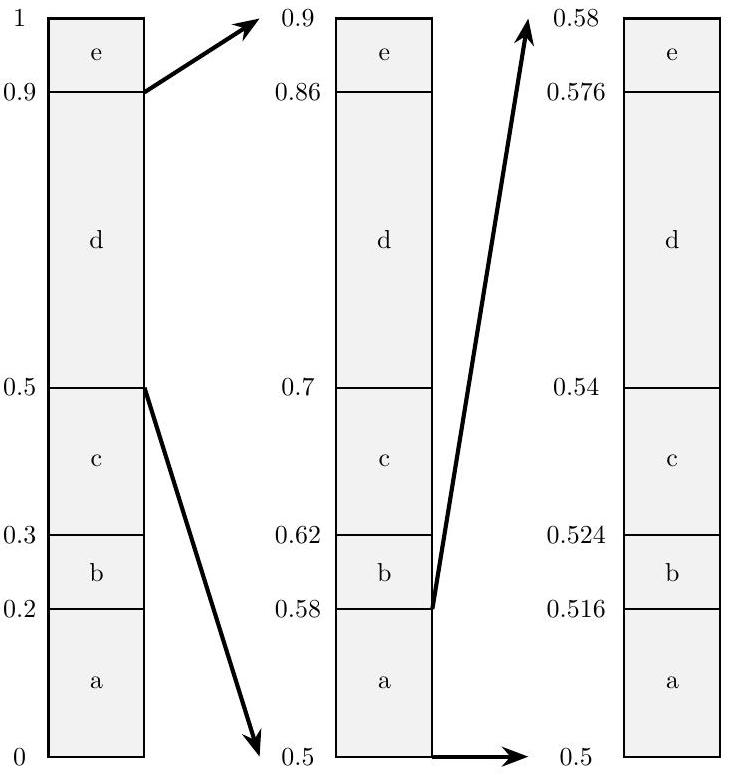
\includegraphics[width=.5\textwidth]{2025_04_25_b5f58c3e8cc704f29fe4g-06}
\caption{Encodage de \lstinline{s = 'dac'}. \label{fig_ccmp_2024_info_02} }
\end{figure}



\question{En considérant la table des fréquences précédente, proposer l'intervalle correspondant à la chaîne \lstinline{s='bac'}.}

On suppose disposer d'une fonction \lstinline{codeCar(car:str, g:float, d:float) -> (float, float)} qui prend en argument un caractère car et les deux extrémités d'un intervalle $[g, d[$ et qui renvoie un tuple composé des extrémités du sous-intervalle de [ $g, d[$ déterminé par le caractère \lstinline{car}. En reprenant l'illustration précédente \lstinline{codeCar('b'0,0,1)} produit \lstinline{(0.2,0.3)} et \lstinline{codeCar('a',0.5,0.9)} produit ( $0.5,0.58$ ).

\question{Écrire une fonction \lstinline{codage(s:str)->(float, float)} prenant en argument la chaîne $s$ et fournissant en réponse le tuple ( $\mathrm{g}, \mathrm{d}$ ) constitué des deux extrémités de l'intervalle [ $g, d[$ produit par l'algorithme de codage précédent.}


Le codage arithmétique consiste alors à coder la chaîne s par un flottant x choisi arbitrairement à l'intérieur de l'intervalle $[g, d[$.

\subsection{Décodage}
Pour effectuer le décodage d'un flottant $\mathbf{x}$, il suffit de repérer dans quelle succession d'intervalles celui-ci se trouve.

À titre d'exemple, reprenons le tableau précédent et considérons le nombre $x=0.123$

\begin{center}
\begin{tabular}{lccccc}
\hline
\textbf{Caractère} & \lstinline{'a'} & \lstinline{'b'}  & \lstinline{'c'} & \lstinline{'d'} & \lstinline{'e'} \\
\hline
\textbf{Fréquence} & 0.2 & 0.1 & 0.2 & 0.4 & 0.1 \\
\hline
\textbf{Intervalle} & $[0 ; 0.2[$ & $[0.2 ; 0.3[$ & $[0.3 ; 0.5[$ & $[0.5 ; 0.9[$ & $[0.9 ; 1[$ \\
\hline
\end{tabular}
\end{center}

Puisque $x$ appartient à l'intervalle $[0 ; 0.2$, le premier caractère est un \lstinline{'a'}. Puisque $x$ appartient au sous-intervalle $[0.10; 0.18[$, le caractère suivant est un \lstinline{'d'}, etc.

\question{Déterminer le caractère qui suit \lstinline{'ad'} dans la chaîne codée par $\mathrm{x}=0.123$ en spécifiant le sous-intervalle qui a permis de décoder ce caractère.}

\question{Dans le cadre de l'exemple de cette partie, indiquer deux chaînes qui peuvent correspondre au flottant 0.2. Expliquer par une phrase ce qui est à l'origine de cette ambiguité.}

Une solution possible pour résoudre le problème précédent consiste à introduire un caractère nouveau signifiant la fin de la chaîne de caractères.

Nous conviendrons de désigner ce caractère par '\#'. Ce caractère se voit attribuer une plage non vide au voisinage de 0 . Dans la suite, on suppose que la table des fréquences est adaptée de sorte à prendre en compte la présence de ce nouveau caractère.

On suppose disposer, en plus de la fonction \lstinline{codeCar(car, g, d)} précédente, d'une fonction \lstinline{decodeCar(x:float, g:float, d:float) -> str} qui détermine le caractère correspondant à la valeur \lstinline{x} quand celle-ci est comprise dans la plage de $[g, d[$.\\
Par exemple \lstinline{decodeCar(0.123,0,1)} donne \lstinline{'a'} tandis que \lstinline{decodeCar(0.123,0,0.2)} donne le caractère \lstinline{'d'}.

\question{Écrire une fonction \lstinline{decodage(x:float) -> str} produisant la chaîne de caractères $\mathbf{s}$ déterminée par la valeur de \lstinline{x} (avec le caractère '\#' compris).}

Le codage précédent ne fonctionne que sous l'hypothèse illusoire d'exactitude des calculs jusqu'à une très grande précision. Cette précision est cependant limitée par la taille de la mantisse représentant un réel et il ne peut être mis en œuvre sous la forme précédente qu'avec des chaînes relativement courtes. Pour résoudre cette difficulté, on adopte un codage en arithmétique entière : au lieu de considérer un intervalle flottant $[0,1[$, c'est un intervalle entier $\llbracket 000 ; 999 \rrbracket$ qui est utilisé. Cette technique ne sera pas abordée dans le cadre de cette épreuve de durée limitée.

\section{Décodage du message reçu par Bob à l'aide de l'algorithme de Viterbi}
\subsection{Modélisation du canal de communication par un graphe}
Dans cette partie, nous allons désormais considérer que le message compressé par Alice a été envoyé au travers d'un canal de communication. À cette fin, et indépendamment de la phase de compression étudiée dans la première partie, le message a subi une deuxième phase de transformation, dite d'encodage (cf Figure 1).

Le message envoyé sur le canal est une suite de symboles à valeurs dans un alphabet, noté $\Sigma$, comportant $K$ symboles. Le choix d'un alphabet efficace n'est pas l'objet de notre étude et constitue un sujet à part entière.

Suite au passage dans le canal de communication, le message envoyé subit une altération de sorte que Bob reçoit une séquence de symboles de $\Sigma$ qui ne correspond pas nécessairement à celle qui a été émise.

Dans cette partie, nous allons voir une approche permettant à Bob de décoder le message reçu et de potentiellement corriger quelques erreurs liées à la transmission du message et à la connaissance a priori de la propension du canal de communication à altérer les symboles du message lors de la transmission.

La modélisation proposée est la suivante :

\begin{itemize}
  \item Bob observe une suite de $N$ symboles $o b s_{0}, \ldots, o b s_{N-1}$, que nous allons représenter par une liste Python $O b s=\left[o b s_{0}, \ldots o b s_{N-1}\right]$,
  \item pour simplifier, on supposera que l'alphabet $\Sigma$ est un ensemble de $K$ entiers consécutifs commençant à 0 , de sorte que $\Sigma=\llbracket 0, K-1 \rrbracket$. Par exemple si $K=3$ et $N=8$, un message valide reçu par Bob pourrait être $[2,0,0,2,1,1,0,0]$.
  \item chacun des symboles observés $o b s_{t}$ correspond à l'altération d'un symbole $s_{t}$ envoyé par Alice. On note $\left[s_{0}, \ldots s_{N-1}\right]$ le message original; pour reprendre l'exemple précédent, Alice pourrait avoir envoyé $[2,0,0,2,1,1,2,0]$.
  \item on connaît, pour chaque paire $(i, j) \in \Sigma^{2}$, la probabilité $E_{i, j}$ que le canal altère le symbole $j$ en un symbole $i$. On stocke ces probabilités dans une liste de listes E ; autrement dit, \lstinline{E[i][j]} est la probabilité conditionnelle d'observer le symbole $i$ sachant que le symbole $j$ a été émis.
\end{itemize}

Ici (par exemple) on pourrait considérer : $E=\left(\begin{array}{ccc}0.7 & 0.2 & 0.3 \\ 0.2 & 0.7 & 0.1 \\ 0.1 & 0.1 & 0.6\end{array}\right)$, représentée par la liste de listes : \lstinline{E=[[0.7,0.2,0.3],[0.2,0.7,0.1],[0.1,0.1,0.6]]}.

Le fait que \lstinline{E[2][0]} vaille 0.1 signifie donc que la probabilité que le symbole observé par Bob soit un 2 sachant qu'Alice a émis un 0 est de 0.1.

\begin{itemize}
  \item on suppose également que le symbole courant $s_{t}$ envoyé par Alice a une incidence sur le symbole suivant $s_{t+1}$ qu'elle peut envoyer, au même titre que dans une langue comme le français, la probabilité d'observer un \lstinline{'t'} dans un mot, n'est pas la même suivant que le caractère précédent est un \lstinline{'e'} ou un \lstinline{'z'}.
\end{itemize}

Ainsi pour chaque couple de symboles $(i, j) \in \Sigma^{2}$, on suppose que l'on connaît la probabilité d'émettre le symbole $j$ à l'instant $t+1$ sachant que symbole $i$ a été émis à l'instant $t$. On suppose également que cette probabilité ne dépend pas de $t$.

L'information concernant ces probabilités de transition d'un symbole à l'autre peut se stocker dans une matrice $P$ de taille $K \times K$, que l'on représente informatiquement par une liste de listes P. Chaque entrée P[i][j] donne la probabilité qu'Alice émette le symbole $j$ à l'instant $t+1$ sachant qu'elle a émis le symbole $i$ à l'instant $t$. En d'autres termes, $\mathrm{P}[\mathrm{i}][\mathrm{j}]=P_{s_{t}=i}\left(s_{t+1}=j\right)$.

On prendra ici à titre d'exemple : $P=\left(\begin{array}{ccc}0.3 & 0.2 & 0.5 \\ 0.4 & 0.4 & 0.2 \\ 0.2 & 0.3 & 0.5\end{array}\right)$, représentée par la liste de listes: \lstinline{P=[[0.3,0.2,0.5],[0.4,0.4,0.2],[0.2,0.3,0.5]]}.

Le fait que \lstinline{P[2][0]} vaille 0.2 signifie donc que la probabilité que le symbole envoyé par Alice à l'instant $t+1$ soit un 0 sachant que celui envoyé à l'instant $t$ est un 2 vaut 0.2 .

Nous allons désormais nous intéresser au problème du décodage : étant donné la liste Obs $=\left[o b s_{0}, \ldots, o b s_{N-1}\right]$ des symboles observés par Bob, quelle séquence $\tilde{s}_{0}, \ldots, \tilde{s}_{N-1}$ est la plus probable?

En d'autres termes, $\tilde{s}_{0}, \ldots, \tilde{s}_{N-1}$ est l'estimation la plus probable faite par Bob du message d'origine $s_{0}, \ldots, s_{N-1}$, étant donné les observations obs $s_{0}, \ldots, o b s_{N-1}$.

La modélisation précédente peut se représenter à l'aide d'un graphe défini comme suit (voir Figure \ref{fig_ccmp_2024_info_03} pour un exemple) :

\begin{itemize}
  \item on crée un sommet $S_{i, j}$ pour chaque symbole possible $0 \leqslant i \leqslant K-1$ et chaque indice d'observation $0 \leqslant j \leqslant N-1$. Chaque couche verticale dans le graphe correspond à un caractère dans le message. Chaque strate horizontale correspond à un symbole.
  \item au niveau de la $j$-ème couche verticale, les sommets $S_{i, j}$ pour $j<N-1$ ont pour successeurs les états $S_{k, j+1}$ pour tous les symboles $k$ possibles,
  \item par commodité, on ajoute un état source $\sigma$ correspondant au début du message décodé et un état cible $\tau$ correspondant à la fin du message, ces états étant respectivement reliés à la première et la dernière couche,
  \item le décodage du message envoyé par Alice correspond à un chemin entre $\sigma$ et $\tau$ dans ce graphe. A chaque sommet du chemin correspond une lettre décodée. Par exemple, le chemin passant par $S_{0,0}, S_{2,1}, S_{0,2}, S_{1,3}$, correspond au décodage de $[0,2,0,1]$.\\
\end{itemize}

\begin{figure}
\centering
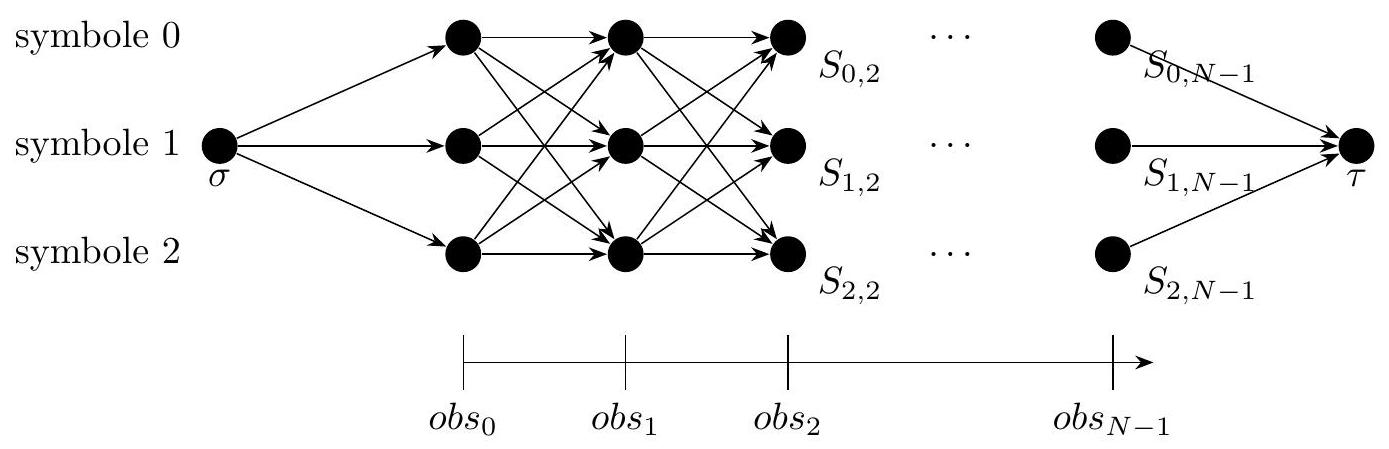
\includegraphics[width=.8\textwidth]{2025_04_25_b5f58c3e8cc704f29fe4g-10}
\caption{Illustration du modèle de décodage considéré ici. \label{fig_ccmp_2024_info_03}}
\end{figure}

À chacune des observations $o b s_{i}$ on peut faire correspondre $K$ états. Chacun de ces états correspond à l'un des symboles potentiellement émis par Alice (ici $K=3$ ). Les états sont organisés en $N$ couches successives. Chaque état est noté $S_{i, j} ; j$ correspond à l'indice dans la suite des symboles émis et $i$ au symbole correspondant. Les états de la couche $j$ et les états de la couche $j+1$ sont reliés par un arc de $j$ vers $j+1$. On ajoute également, par commodité, un état source $\sigma$ et un état cible $\tau$ respectivement reliés à la première et à la dernière couche.

\question{En fonction de $N$ et de $K$, donner le nombre de sommets et d'arcs du graphe illustré par la Figure 3. On ne comptera pas les sommets source $\sigma$ et cible $\tau$, ni les arcs partant du sommet source $\sigma$ ni ceux arrivant à la cible $\tau$.}

On choisit désormais de pondérer chaque arc par la probabilité de transiter par cet arc. Autrement dit :

\begin{itemize}
  \item les arcs issus de la source $\sigma$ vers $S_{i, 0}$ sont pondérés par $E_{\text {obso }, i}$ la probabilité d'observer le symbole $o b s_{0}$ sachant que le symbole $i$ a été émis par Alice;
  \item les arcs arrivant à la cible $\tau$ sont pondérés par 1 (en fin de message, on transite forcément vers l'état final),
  \item les arcs internes entre $S_{i, j}$ et $S_{k, j+1}$ sont pondérés par la probabilité $E_{o b s_{j+1}, k} P_{i, k}$.
\end{itemize}

La probabilité d'un chemin $\sigma S_{i_{0}, 0} S_{i_{1}, 1} \ldots S_{i_{N-1}, N-1} \tau$ entre $\sigma$ et $\tau$ est le produit des probabilités des arcs qui le composent.

L'objectif va être de trouver le chemin de probabilité maximale dans ce graphe entre le sommet source $\sigma$ et le sommet cible $\tau$.\\[0pt]

\question{On suppose que Bob a observé la séquence [2,0]. En utilisant les matrices E et P données dans l'énoncé (avec $K=3$ ), construire le graphe pondéré associé à ce message de longueur $N=2$. Les arcs entre les sommets devront être pondérés par les probabilités correspondantes.}

\question{On revient dans le cas général, $N$ et $K$ sont désormais quelconques. Indiquer combien il existe de chemins entre $\sigma$ et $\tau$ (un ordre de grandeur utilisant la notation $O$ ou $\Theta$ est accepté). Préciser si un algorithme d'exploration exhaustive est envisageable dans ce cas.}

\subsection{Stratégie gloutonne}
Pour pouvoir implémenter correctement la recherche du chemin de probabilité maximale, il est utile de disposer d'une fonction auxiliaire qui sera utilisée dès que nécessaire.

\question{Pour une liste liste, on appelle argument du maximum et on note argMax tout indice $i$ tel que \lstinline{liste[i]} soit maximal. Proposer une fonction \lstinline{maximumListe(liste: [float])->(float,int)} qui prend en entrée une liste de nombres et qui renvoie la valeur du maximum de la liste ainsi que le plus petit argument du maximum, i.e. le premier indice auquel cette valeur maximale apparaît.}

On souhaite appliquer un algorithme glouton pour trouver le chemin de probabilité maximale entre le sommet source $\sigma$ et le sommet cible $\tau$. On rappelle qu'un algorithme glouton cherche, à chaque étape, à faire le choix localement optimal. Ici, si à une étape on se retrouve au sommet $S_{i, j}$, il s'agit de choisir l'arc de plus forte probabilité partant de ce sommet.

Dans un premier temps on écrit une fonction
\lstinline{initialiserGlouton(Obs:[[int]], E:[[float]], K:int) -> int} qui permet d'initialiser l'algorithme glouton en trouvant le sommet le plus probable parmi $S_{i, 0}$ pour $i$ variant entre 0 et $K-1$. Pour cela il faut regarder la colonne \lstinline{Obs[0]} de \lstinline{E} et relever l'indice de la plus grande valeur.

\begin{lstlisting}
def initialiserGlouton(Obs, E, K):
    probasInitiales = [E[Obs[O][i]] for i in range(K)]
    s, symbole = maximumListe(probasInitiales)
    return symbole
\end{lstlisting}


\question{Proposer une fonction \lstinline{glouton(Obs:[int], P:[[float]],E:[[float]],K:int,N:int) -> [int]} qui renvoie la liste d'états obtenue par l'approche gloutonne. Même si cela n'est pas nécessaire, $K, N$ seront des arguments de cette fonction.}


\question{En fonction de $K$ et de $N$, quelle est, en ordre de grandeur, la complexité temporelle asymptotique de l'approche gloutonne?}

\question{Indiquer le chemin renvoyé par l'algorithme glouton appliqué à la Figure \ref{fig_ccmp_2024_info_04}. Conclure quant à l'optimalité de l'approche.}

\begin{figure}
\centering
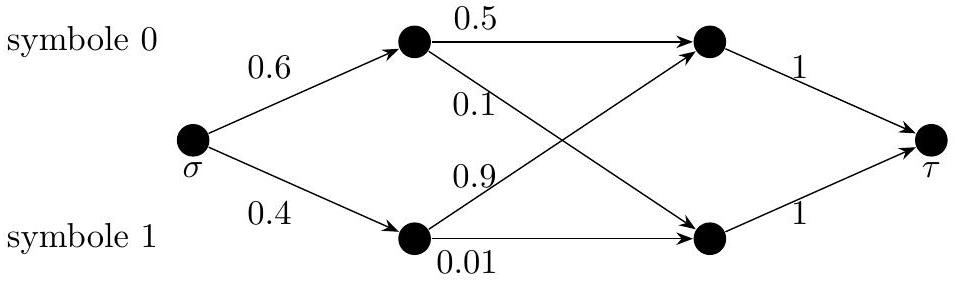
\includegraphics[width=.8\textwidth]{2025_04_25_b5f58c3e8cc704f29fe4g-11}
\caption{Que donne l'algorithme glouton ici~? \label{fig_ccmp_2024_info_04}}
\end{figure}




\subsection{Stratégie de programmation dynamique}

\question{Expliquer en quoi rechercher un chemin de probabilité maximale pourrait se transformer en un problème de recherche de plus court chemin dans un graphe pondéré à poids positifs. Préciser alors quel algorithme pourrait être utilisé.}

Les algorithmes évoqués à la question précédente ne sont cependant pas optimaux dans ce cas. L'algorithme optimal est dû à Andrew Viterbi et date de 1967. Il repose sur le paradigme de la programmation dynamique.

On appelle $T_{i, j}$ la valeur de probabilité maximale entre la source et l'état $S_{i, j}$. On peut alors établir l'équation de programmation dynamique suivante :

$$
\left\{\begin{array}{l}
T_{i, j}=\max _{k \in[0, K-1 \rrbracket}\left\{T_{k, j-1} \times P_{k, i} \times E_{o b s}, i\right\} \text{ si } N-1 \geq j > 0  \\
T_{i, 0}=E_{o b s_{0}, i}
\end{array}\right.
$$

Comme on cherche également à obtenir la valeur des états correspondant au chemin optimal, on maintient également le tableau des prédécesseurs suivant :

$$
\left\{\begin{array}{l}
\arg T_{i, j}=\underset{k \in[0, K-1]}{\arg \max }\left\{T_{k, j-1} \times P_{k, i} \times E_{o b s, j}, i\right. \\
\arg T_{i, 0}=-1
\end{array}\right.
$$

La valeur \lstinline{-1} du deuxième tableau est purement conventionnelle et ne sert qu'à représenter l'état source $\sigma$ qui ne correspond pas à une observation.

On suppose avoir codé une fonction \lstinline{initialiserViterbi(E:[[float]], Obs0:int, K:int, N:int)->([[float]],[[int]])} qui prend en entrée la matrice E d'émission, la valeur de la première observation \lstinline{ObsO}, le nombre d'éléments \lstinline{K} de $\Sigma$, le nombre d'observations N et qui renvoie deux tableaux (liste de listes) T et argT vérifiant les caractéristiques suivantes :

\begin{itemize}
  \item \lstinline{T} et \lstinline{argT} sont de dimensions $K$ lignes par $N$ colonnes;
  \item \lstinline{T[i] [0]} contient la valeur de $E_{o b s_{0}, i}$;
  \item \lstinline{argT[i][0]} contient la valeur $-1$;
  \item les autres valeurs de \lstinline{T} et\lstinline{argT} sont à 0 .
\end{itemize}

En voici une implémentation possible :

\begin{lstlisting}
def initialiserViterbi(E, ObsO, K, N):
    probasInitiales = [E[Obs0][i] for i in range(K)]
    T = [[0 for j in range(N)] for i in range(K)]
    argT = [[0 for j in range(N)] for i in range(K)]
    for i in range(K):
        T[i][0] = probasInitiales[i]
        argT[i][0] = -1
    return T, argT
\end{lstlisting}

\question{Proposer une fonction (méthode de bas en haut de programmation dynamique) \lstinline{construireTableauViterbi(Obs:[int], P:[[float]], E:[[float]], K:int, N:int)
-> ([float]], [[int]])} qui prend comme arguments la liste des observations Obs, la matrice des probabilités de transition $P$ et la matrice des probabilités \lstinline{E} et renvoie les deux listes de listes \lstinline{T} et \lstinline{argT} de taille $K \times N$.}

\question{L'algorithme de Viterbi codé en Python et appliqué à un message en entrée
donne les tableaux \lstinline{T} et \lstinline{argT} suivants. Indiquer la séquence d'états la plus probable.}

$$
\begin{gathered}
T=\left(\begin{array}{cccccccc}
0.1 & 0.084 & 0.018 & 0.00053 & 0.00021 & 8.9 e-05 & 8.7 e-05 & 1.8 e-05 \\
0.1 & 0.036 & 0.0054 & 0.00041 & 0.0011 & 0.00031 & 2.5 e-05 & 3.5 e-06 \\
0.6 & 0.09 & 0.014 & 0.0053 & 0.00026 & 2.2 e-05 & 1.9 e-05 & 1.3 e-05
\end{array}\right) \\
\\
\arg T=\left(\begin{array}{cccccccc}
-1 & 2 & 0 & 0 & 2 & 1 & 1 & 0 \\
-1 & 2 & 2 & 2 & 2 & 1 & 1 & 0 \\
-1 & 2 & 0 & 0 & 2 & 1 & 1 & 0
\end{array}\right)
\end{gathered}
$$

\question{En fonction de $K$ et de $N$, donner l'ordre de grandeur de la complexité temporelle de l'approche de programmation dynamique, ainsi que la complexité spatiale.}

